\chapter{RNA Base-Pairs}
\label{basepairs} 
\bibliographystyle{nar}
\section{Canonical and Non-canonical Base-Pairs}
As  shown  in  Figure  \ref{fig:saenger28},  there  is  a  variety  of
base-pairing patterns between the  heterocyclic bases in nucleic acids
due  to the  many possible  hydrogen bonding  interactions.   The most
prevalent hydrogen  bonding pattern  in nucleic acids  is that  of the
canonical  Watson-Crick (WC)  base-pair.  Patterns  other than  the WC
pairs are known as non-canonical base pairs and are more common in RNA
than in DNA.  We used  the 3DNA \cite{lu2003} software package to find
all base  pairs in a  non-redundant dataset of RNA  crystal structures
with resolution better than 3.5  \AA~ downloaded from the Protein Data
Bank (PDB).  We also constrained  our search to helical regions, which
are  defined  as stretches  of  three  or  more spatially  consecutive
base-pairs which need not  be covalently bonded by the sugar-phosphate
backbone between sequentially consecutive base pairs \cite{olson2009}.

\begin{table}[htbp]
\begin{center}
\begin{tabular}{|l|c|r|r|r|r|}
\hline
RNA Type & \multicolumn{1}{p{2cm}|}{Number of Structures} & \multicolumn{1}{c|}{G} &
\multicolumn{1}{c|}{C} & \multicolumn{1}{c|}{A} &
\multicolumn{1}{c|}{U} \\ \hline 
small helices & 78 & 36 & 30 & 16 & 18 \\ \hline
drug-RNA & 36 & 36 & 33 & 14 & 17 \\ \hline
protein-RNA & 207 & 37 & 32 & 16 & 16 \\ \hline
protein-tRNA & 9 & 34 & 30 & 19 & 17 \\ \hline
rRNA & 13 & 37 & 28 & 18 & 17 \\ \hline
tRNA & 13 & 34 & 27 & 21 & 19 \\ \hline
ribozyme & 113 & 34 & 29 & 20 & 16 \\ \hline
Total & 469 & \multicolumn{1}{c|}{36} & \multicolumn{1}{c|}{30} & \multicolumn{1}{c|}{18} & \multicolumn{1}{c|}{16} \\ \hline
\end{tabular}
\caption{Description  of the  types  of RNA  structures  and the  base
  content of  each group in  the non-redundant dataset of  RNA crystal
  structures with resolution better than 3.5 \AA given as a percentage
  of  the total  number of  structures  per group.   The listed  bases
  comprise  the base  pairs in  helices of  three or  more base-pairs.
  Further detail on the structures which compose the dataset including
  PDB\_ID's  and NDB\_ID's  can  be obtained  online as  supplementary
  material attached to Olson et al. \cite{olson2009} results.}
\label{tab:dbase}
\end{center}
\end{table}

Our dataset is non-redundant in the sense that from the main source of
RNA structural information, which is the ribosome, we used only one of
the  available structures  per  organism,  that is,  one  for each  of
\textit{Deinococus   radiodurans},   \textit{Haloarcula  marismortui},
\textit{Escherichi          coli},         and         \textit{Thermus
  thermophilus}. Table~\ref{tab:dbase}  shows in detail  the number of
bases for each  RNA type in our dataset of  helical structures.  It is
interesting to see  that in general the content of G  and C, is higher
than that  of A  and U. The  difference might  be related to  a higher
overall  stability  of  G$\cdot$C  base-pairs  compared  to  A$\cdot$U
base-pairs.

In  Table  \ref{tab:bpcomp}  we  show  the  number  of  base-pairs  of
different  chemical  types formed  by  unmodified  nucleotides in  our
dataset,  it is  clear from  the  table that  G$\cdot$C and  A$\cdot$U
base-pairs  dominate the  RNA  base-pairs formed  in helical  regions,
making up 80\% of all the base-pairs. If we count only those that form
canonical  WC base-pairs  (9500  G$\cdot$C, and  3069 A$\cdot$U),  the
number corresponds to 73\% of all base-pairs in helical regions.

As will  be show later (Table~\ref{tab:seven}),  a considerable number
of the A$\cdot$U's  pairs associate in a Hoogsteen  arrangement. A few
of these examples form  U$\cdot$A$\cdot$U triplets containing a WC and
a   Hoogsteen  \footnote{Hoogsteen   base-pairs  are   illustrated  by
  structure XXIII of the Saenger classification of base-pairs as shown
  in Figure~\ref{fig:saenger28}} base pair in the RNA helical regions.

\begin{table}[htbp]
\begin{center}
\begin{tabular}{|c|c|c|c|c|}
\hline
A    &      G    &      C    &      U    &      B/B$'$ \\ \hline
384  &    980    &    313    &   3975    &      A  \\ \hline
     &    128    &   9913    &   1282    &      G  \\ \hline
     &           &     63    &    103    &      C  \\ \hline
     &           &           &    187    &      U  \\ \hline
\end{tabular}
\caption{Composition  of base  pairs in  the  non-redundant structural
  dataset. Note that 9500 out of 9913 G$\cdot$C and 3069
  out of  3975 A$\cdot$U  are canonical WC  base pairs. See  legend to
  Table \ref{tab:dbase} for dataset details.}
\label{tab:bpcomp}
\end{center}
\end{table}

\subsection{RNA Base-Pairs Classification}
We classified the RNA base  pairs in our dataset using three criteria:
(1) the Leontis-Westhof edge classification scheme \cite{leontis1998},
which is based on the  identities of the three major interacting edges
for  hydrogen-bond formation  called the  WC (W),  Hoogsteen  (H), and
Sugar  (S)  edges, (2)  the  rotational  and translational  rigid-body
base-pairing  parameters  called,  shear,  stretch,  stagger,  buckle,
propeller and opening,  and (3) the location of  the base-pairs within
the helices,  that is, their location in  either ``intact'' covalently
bonded   sugar-phosphate  backbones  or   within  ``quasi-continuous''
helices  with  breaks  in   the  sugar-phosphate  backbone  and  their
positions within these kinds of helices (see below).

We find  that $\sim$90\% of the base  pairs in the RNA  helices in our
dataset  form base  pairs in  one of  seven  possible hydrogen-bonding
types; canonical  WC G$\cdot$C and A$\cdot$U  pairs, and non-canonical
G$\cdot$U  wobble,  sheared G$\cdot$A,  Hoogsteen  A$\cdot$U, WC  type
G$\cdot$A, and  U$\cdot$U wooble base pairs.  Detailed results showing
how these seven major  RNA base-pairing types are classified according
to various  schemes, and the details of  their hydrogen-bond distances
is given in Table~\ref{tab:seven} and in Figure~\ref{fig:pairs}

\begin{figure}[ht]
\centering
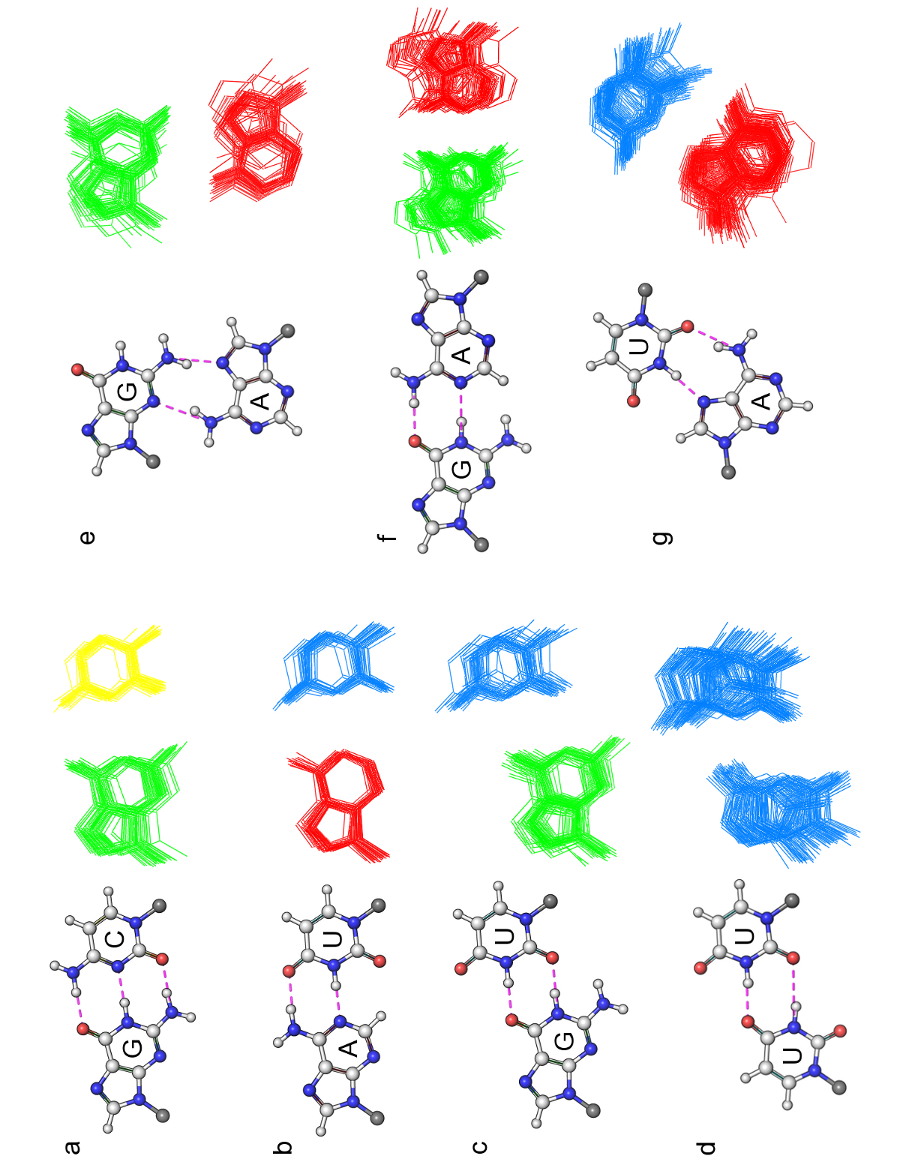
\includegraphics[angle=-90, scale=0.75]{Chapter3/sevenpairs.png}
\caption{Seven most prominent base pairs in RNA helical regions in our
  structural  dataset  shown  in  images (a-g),  (a-b)  the  canonical
  G$\cdot$C and A$\cdot$U Watson-Crick pairs, (c) the wobble G$\cdot$U
  pair, (d) the wobble U$\cdot$U pair, (e) the sheared G$\cdot$A pair,
  (f)  the Watson-Crick-like  G$\cdot$A  pair, and  (g) the  Hoogsteen
  A$\cdot$U pair.  The images on  the left for each base-pair show the
  identities  of the  bases, atom  types (oxygen  red,  nitrogen blue,
  carbon  and   hydrogen  white,  and  C1$'$  atoms   gray),  and  the
  hydrogen-bond  connectivity  (magenta  colored dashed  lines).   The
  rigth  side   images  of   each  base-pair  representation   show  a
  superposition of the base pairs  in our helical dataset, centered in
  the middle  base triad  (MBT) reference frame  (The definition  of a
  middle base triad  is completely analogous to that  of a middle step
  triad as explained thoroughly in Appendix \ref{appendix_1a}).}
\label{fig:pairs}
\end{figure}

\begin{sidewaystable}
\begin{center}
\begin{tabular}{|c c|c c|c|c|c c|c|}
\hline
Base-pair & & Hydrogen bonds &  & Sign & Saenger & Leontis-Westhof & &
Number \\
\hline
\hline
\multicolumn{9}{|l|}{Canonical} \\
\hline
G$\cdot$C & Watson-Crick & N2-H$\cdots$O2 & 2.79(0.17) & - & XIX & cis
 & W/W & 9500$_{\text{x0.90}}$ \\
 & & O6$\cdots$H-N4 & 2.92(0.18) & & & & &  \\
 & & N1-H$\cdots$N3 & 2.89(0.13) & & & & &  \\
\hline
A$\cdot$U & Watson-Crick & N1$\cdots$H-N3 & 2.84(0.14) & - & XX & cis
& W/W & 3069$_{\text{x0.93}}$ \\
 & & N6-H$\cdots$O4 & 2.97(0.18) & & & & &  \\
\hline
\multicolumn{9}{|l|}{Non-canonical} \\
\hline
G$\cdot$U & Wobble & N1-H$\cdots$O2 & 2.79(0.16) & - & XXVIII & cis
 & W/W & 1049$_{\text{x0.69}}$ \\
 & & O6$\cdots$H-N3 & 2.85(0.16) & & & & &  \\
\hline
G$\cdot$A & Sheared & N2-H$\cdots$N7 & 2.89(0.17) & + & XI & trans
 & H/S & 509$_{\text{x0.59}}$ \\
 & & N3$\cdots$H-N6 & 3.03(0.18) & & & & &  \\
\hline
A$\cdot$U & Hoogsteen & N6-H$\cdots$O2 & 2.91(0.21) & + & XXIII & trans
 & H/W & 354$_{\text{x0.71}}$ \\
 & & N7$\cdots$H-N3 & 2.90(0.17) & & & & &  \\
\hline
G$\cdot$A & Watson-Crick & N1-H$\cdots$N1 & 2.84(0.17) & - & VIII & cis
 & W/W & 185$_{\text{x0.85}}$ \\
 & & O6$\cdots$H-N6 & 2.91(0.20) & & & & &  \\
\hline
U$\cdot$U & Wobble & O2$\cdots$H-N3 & 2.95(0.24) & - & XVI & cis
 & W/W & 141$_{\text{x0.54}}$ \\
 & & N3$\cdots$H-O4 & 2.87(0.15) & & & & &  \\
\hline
\end{tabular}
\caption{Seven  dominant  base-pairing  types  found  in  RNA  helical
regions.   The  first  column   lists  the  Gutell  and  collaborators
nomenclature \cite{lee2004}  of the base  pairs. Column two  shows the
standard  hydrogen bonding  pattern  associated with  each base  pair.
Column  three  displays a  negative  sign  if  the bases  forming  the
base-pair oppose each other and a positive sign if they share the same
face \cite{lu2003}.   Column four gives the  Saenger classification as
in Figure \ref{fig:saenger28}.   Column five lists the Leontis-Westhof
edge    classification   obtained    trough   the    RNAVIEW   program
\cite{yang2003},  and  the  last  column  gives the  total  number  of
identified base  pairs of  each category and  the percentage  of those
which comply exactly with the hydrogen-bonding pattern shown in column
two.}
\label{tab:seven}
\end{center}  
\end{sidewaystable}  


\subsection{Base-Pairs in Helical Regions}
Our classification also includes the locations of the base pairs in helical
regions, that is,  whether they are in the interior or  at the ends of
``intact'' or ``quasi-continuous'' helical
regions.  Figure~\ref{fig:helregxin}  illustrates  the  two  types  of
helical regions  mentioned. The ``intact'' helical region
is depicted in Figure \ref{fig:helregxin}a.
The ``quasi-continuous'' helical region shown in Figure \ref{fig:helregxin}b.

\begin{figure}
\centering
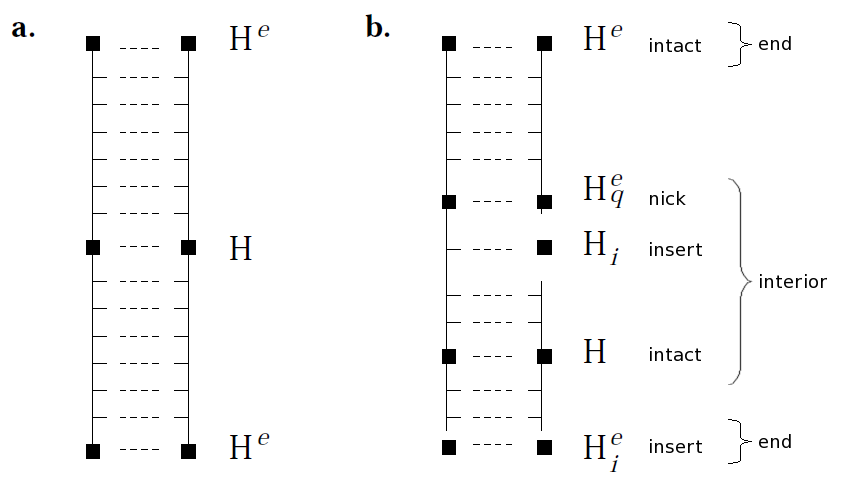
\includegraphics[scale=0.4]{Chapter3/helcontext.png}
\caption{(a)  Intact  and  (b)  quasi-continuous  helical  regions  in
  RNA. Image kindly provided by Dr. Yurong Xin.}
\label{fig:helregxin}
\end{figure}  

The locations of  the base pairs in helical  regions are summarized in
Table~\ref{tab:helcontext}.     The     A$\cdot$U    Hoogsteen    pair
(A$\cdot$U$_{\text{H}}$)  stands out  as  being present  mainly as  an
insert   \footnote{Similar   to    the   way   intercalating   ligands
  (intercalators)  insert  themselves  in  DNA.} in  helical  regions,
sometimes in nicked  regions and rarely in intact  ones. The G$\cdot$A
Watson-Crick-like  pair  (G$\cdot$A$_{\text{WC}}$)  differs  from  the
A$\cdot$U  Hoogsteen pair,  in that,  it rarely  occurs as  an insert,
preferring to be in nicks,  and sometimes in intact regions. A similar
situation     happens    with     the    sheared     G$\cdot$A    pair
(G$\cdot$A$_{\text{s}}$), which also rarely occurs as an insert and is
mainly found in intact regions, and sometimes in nicks.  The canonical
WC G$\cdot$C base-pair is two times more likely to occur at the end of
helical regions than the canonical A$\cdot$U base-pair.  The
helical context of  the G$\cdot$U wobble pair (G$\cdot$U$_{\text{w}}$)
is quite similar to that of the canonical base-pairs, with location more closely
resembling  the  context  of  G$\cdot$C$_{\text{WC}}$,  than  that  of
A$\cdot$U$_{\text{WC}}$.  The G$\cdot$U wobble  stands out from the WC
base pairs  in being  slightly more prevalent  in nicked  regions. The
G$\cdot$U$_{\text{w}}$ pair is similar to the canonical A$\cdot$U pair
in that is more commonly seen in
interior  regions  than  in  ends.  Because of  the  large  number  of
G$\cdot$C WC  base pairs its helical context  is practically identical
to the one given for all base-pairs.

\begin{table}[htbp]
\begin{center}
\begin{tabular}{|c|c|c|c|c|c|c|c|c|}
\hline
Helical context & \multicolumn{8}{c|}{Base-pair} \\
\hline
 & All & G$\cdot$C$_{\text{WC}}$ & A$\cdot$U$_{\text{WC}}$ &
G$\cdot$U$_{\text{w}}$ & G$\cdot$A$_{\text{s}}$ &
A$\cdot$U$_{\text{H}}$ & G$\cdot$A$_{\text{WC}}$ &
U$\cdot$U$_{\text{w}}$  \\
\hline
\multicolumn{9}{|c|}{Interior} \\
\hline
Intact &  0.62 & 0.62 & 0.75 & 0.63 & 0.34 & 0.05 & 0.25 & 0.74 \\
Nick   &  0.20 & 0.20 & 0.16 & 0.26 & 0.25 & 0.29 & 0.66 & 0.13 \\
Insert &  0.02 & 0.01 & 0.01 & 0.00 & 0.00 & 0.42 & 0.01 & 0.03 \\
\hline
\multicolumn{9}{|c|}{Ends} \\
\hline
Intact &  0.13 & 0.15 & 0.07 & 0.10 & 0.33 & 0.05 & 0.06 & 0.10 \\
Insert &  0.02 & 0.01 & 0.01 & 0.01 & 0.05 & 0.19 & 0.02 & 0.00 \\
\hline
\end{tabular}
\caption{Distribution of helical location of the seven most abundant
  base-pairs in  our RNA helical regions dataset.  The helical context
  is  shown in  a secondary  structure representation  in Figure
  \ref{fig:helregxin}.}
\label{tab:helcontext}
\end{center}
\end{table}

The mean length of the helical domains in our dataset is 11 base pairs
as   shown  in   the  histogram   of  helix   length   frequencies  in
Figure~\ref{fig:hellength}.  The value of 11 base pairs coincides with
the  number  of   residues  per  turn  in  a   canonical  A-RNA  fiber
\cite{arnott1968}   which   indicates   that   the   canonical   A-RNA
conformation  is  predominant,  and   is  most  likely  maintained  by
canonical  WC pairs  which  constitute  73\% of  all  base pairs.   In
accordance with Leontis  and collaborators work \cite{nasalean2009} we
see that helices are usually  short and less frequently longer than 15
residues. In contrast to their findings we feel it's important to note
that  the total  number  of helices  longer  than 15  residues is  not
negligible.

\begin{figure}
\centering
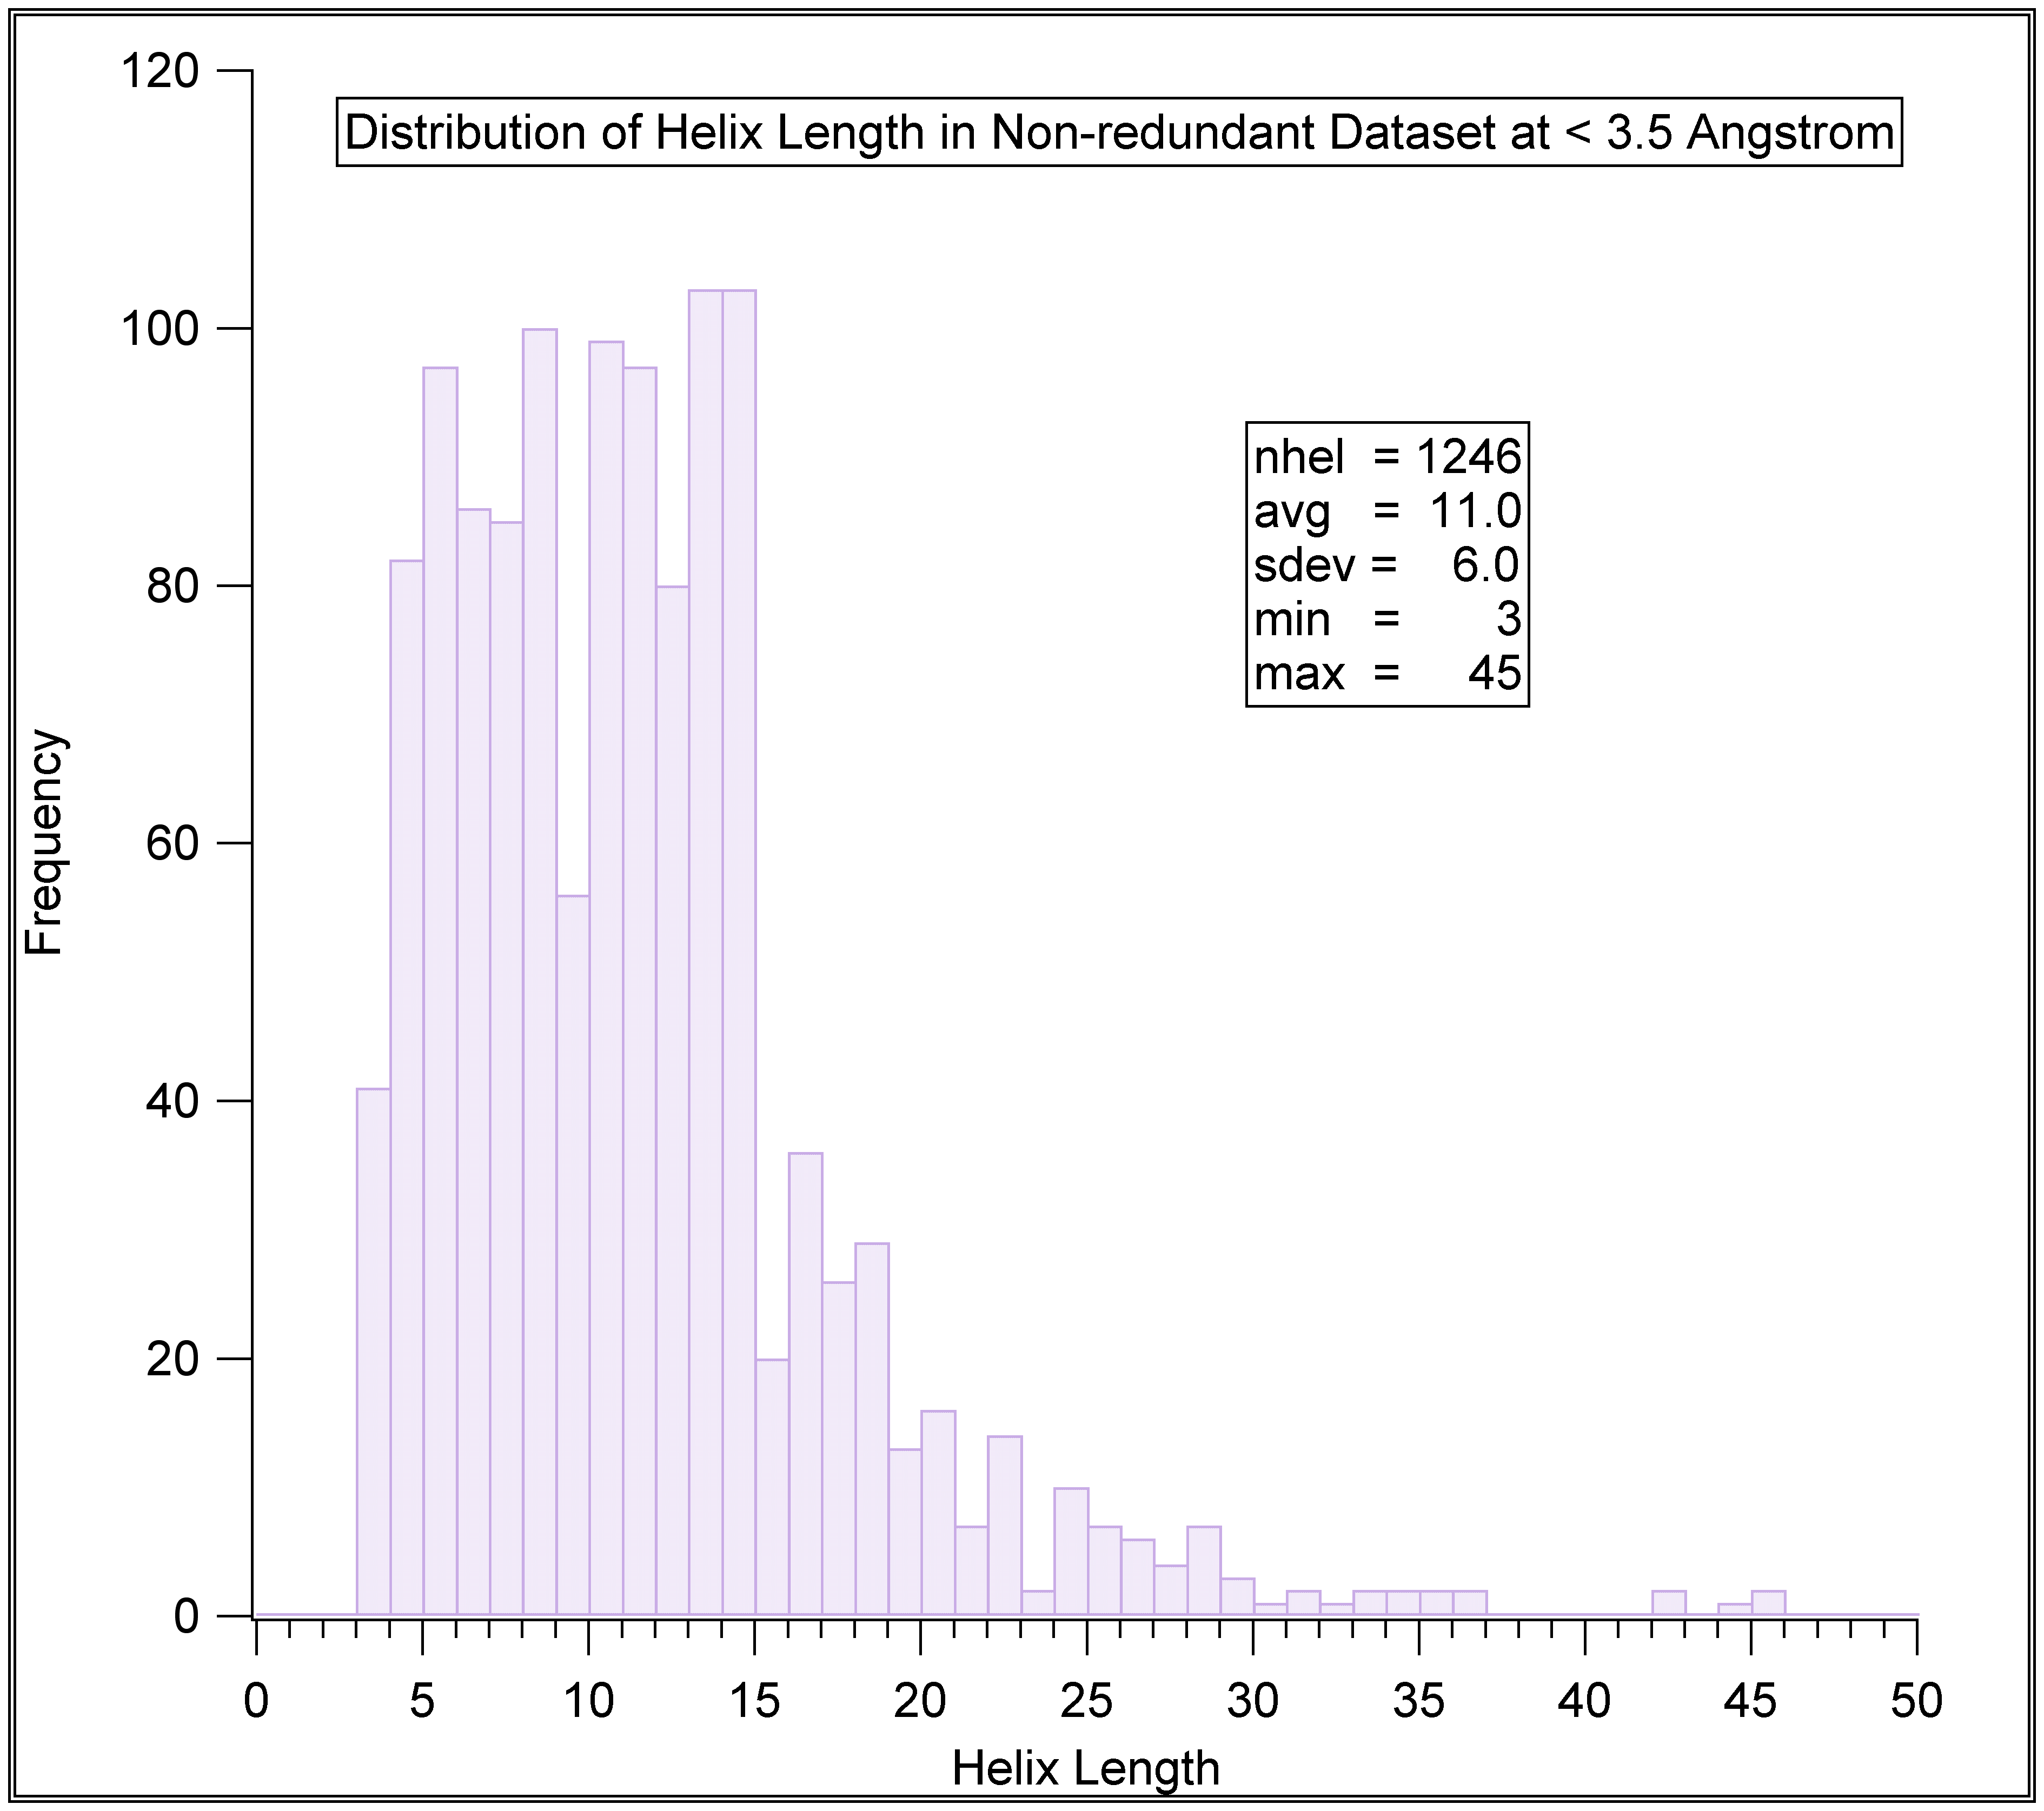
\includegraphics[angle=0, scale=0.5]{Chapter3/heldistrib.png}
\caption{Histogram showing the distribution  of helical regions in our
  non-redundant   helical  dataset   composed   of  structures   whose
  resolution  is better  than 3.5  \AA.  The  total number  of helices
  (nhel),  the average  helix  length (avg),  it's standard  deviation
  (sdev), and the  minimum (min) and maximum (max)  helix lenghts are
  given in the legend.}
\label{fig:hellength}
\end{figure}


\section{Deformability of Base-Pairs}
Figure   \ref{fig:pairs}  shows   a  visual   representation   of  the
deformability of the seven most  predominant base pairs in RNA helical
regions. The overlapping structures for each base-pair are centered in
the middle  base triad  (see Appendix for  \ref{appendix_1a} details).
In  Table \ref{tab:bppar}  we have  collected the  averages  and their
corresponding  standard deviations  for the  rigid-body  parameters of
base pairs, along with a  deformability score, which is extracted from
the  covariance  of   the  rigid-body  parameters.  Specifically,  $V$
\cite{olson1998} is  given by the product  of the square  roots of the
eigenvalues  of  the  base-step  parameters covariance  matrix.   Thus
volume   scores   correspond    to   the   accessible   conformational
volume.   Table  \ref{tab:bppar}   also  lists   the  root-mean-square
deviation (rmsd) of the  structures which have been superimposed using
the middle base triad of the base pairs. The rmsd reported is the mean
value  of  rmsd's  for  all  base pairs  in  the  predominant  groups.
Furthermore,  this  rsmd values  are  computed  between the  cartesian
coordinates  of  all atoms  in  a base  pair  and  the average  atomic
cartesian coordinates of all base pairs in a group \cite{eargle2006}.

As seen  from Table \ref{tab:bppar}, the  non-canonical base-pairs are
clearly more deformable  than the canonical WC base-pairs  in terms of
their volume  scores and rmsd values. This  larger deformability comes
mainly  from the  in-plane parameters,  that is,  Shear,  Stretch, and
Opening,   which  determine   the   hydrogen-bonding  patterns.    The
out-of-plane  parameters Stagger,  Buckle, and  Propeller  are roughly
comparable to  those of  the less deformable  WC base-pairs.  That is,
there is more deformability in the non-canonical pairs at the level of
hydrogen-bonding  controlling parameters,  and  less at  the level  of
planarity controlling  ones. Another  fact that confirms  this greater
variability  is  the  smaller  fraction  of  base-pairs  which  comply
strictly to the standard hydrogen bonding pattern in non-canonical vs.
canonical  base   pairs,  as  seen   in  the  last  column   of  Table
\ref{tab:seven}.

For example  whereas 90  percent of the  canonical WC  G$\cdot$C which
complies to the binding pattern shown in column three, only 54 percent
of  the  U$\cdot$U  wobble  base  pairs associate  strictly  with  the
standard O2$\cdots$H-N3 and N3- H$\cdots$O4 interacting pattern.

What's  occurring with the  additional non-canonical  base-pairs which
are not included  in the hydrogen-bond distance averages  is that they
are  ``melting'', that  is,  the WC  pairs,  as defined  here, do  not
include such melted states which  are forming fewer hydrogen bonds, or
different  types of  heavy  atom bridges  mediated  by hydrogen.   The
combination of  angular and translational  parameters, with respective
units   in  degrees  and   Angstroms,  makes   the  analysis   of  the
conformational  volume score  complicated.   Nonetheless, the  general
trends give  a clear indication  of three main levels  of deformation.
That  is, canonical  G$\cdot$C and  A$\cdot$U base  pairs with  a mean
score   of    4.5   are   not   very   deformed    compared   to   the
G$\cdot$U$_{\text{w}}$,           G$\cdot$A$_{\text{s}}$,          and
A$\cdot$U$_{\text{H}}$ pairs  with mean values  of around 25,  and the
remaining U$\cdot$U$_{\text{w}}$  and G$\cdot$A$_{\text{WC}}$ are more
deformable   than   any   other   pairs.    A   more   straightforward
interpretation  of  spatial deformability  comes  from  the root  mean
square deviation (rmsd)  values of the base pair  groups. These values
are  computed by  reconstructing all  atom base-pair  structures using
their base-pair parameters.  The rmsd values are then obtained from an
all-atom  superposition  of  base-pairs  aligned  with  respect  their
standard base-pair reference frames and then the average rmsd value is
computed with respect to the mean structure. The rmsd values have been
obtained  using  the  vmd  software  package  \cite{eargle2006}.   The
deformability  of   base-pairs  as   ranked  by  their   rmsd  values,
U$\cdot$U$_{w}$  (0.74 \AA)  > G$\cdot$A$_{WC}$  (0.54  \AA) $\approx$
G$\cdot$A$_{s}$  (0.50  \AA) >  G$\cdot$U$_{w}$  (0.45 \AA)  $\approx$
A$\cdot$U$_{H}$  (0.43 \AA)  > G$\cdot$C$_{WC}$  (0.38  \AA) $\approx$
A$\cdot$U$_{WC}$ (0.36 \AA) does not  follow exactly the same trend as
that of the conformational  volume score.  The rmsd values nonetheless
roughly maintain  the ordering of  the three levels  of deformability,
although from  this perspective the  G$\cdot$A$_{\text{WC}}$ base pair
may   be   better   grouped   with  the   intermediate   deformability
non-canonical steps.  An interesting  observation is the prominence of
the    base-pair     with    the    greatest     deformability,    the
U$\cdot$U$_{\text{w}}$ base-pair, is more prominent in the interior of
intact helical  regions, compared to  the location of  less deformable
non-canonical pairs,  which show a  preference for nicked  or inserted
regions in RNA helical regions.

\begin{sidewaystable}[htbp]
\begin{center}
\begin{tabular}{|c|c|c|c|c|c|c|c|c|}
\hline
Base-pair & \multicolumn{8}{c|}{Rigid-body parameters} \\
\hline
 & Shear (\AA) & Stretch (\AA) & Stagger (\AA) & Buckle (deg) &
Propeller (deg) & Opening (deg) & V (deg$^{\text{3}}$
\AA$^{\text{3}}$) & rmsd \\
\hline
G$\cdot$C$_{\text{WC}}$ & -0.20 (0.41) & -0.15 (0.17) & -0.04 (0.40) & -3.4 (8.4)  &  -8.7  (8.5) &  0.5  (4.5)  & 6.5   & 0.38\\
A$\cdot$U$_{\text{WC}}$ &  0.04 (0.34) & -0.14 (0.15) &  0.04 (0.39) & -0.3 (8.4)  &  -9.0  (8.7) &  0.9  (5.2)  & 6.4   & 0.36\\
G$\cdot$U$_{\text{w}}$  & -2.11 (0.84) & -0.52 (0.27) & -0.04 (0.43) & -0.1 (8.2)  &  -7.4  (7.5) & -0.6  (6.9)  & 25.1  & 0.45\\
G$\cdot$A$_{\text{s}}$  &  6.78 (0.23) & -4.40 (0.55) &  0.14 (0.52) &  1.5 (11.0) &  -3.2  (9.1) & -5.3  (8.2)  & 27.2  & 0.50\\
A$\cdot$U$_{\text{H}}$  & -4.06 (0.80) & -1.92 (0.84) &  0.07 (0.61) & -0.4 (7.3)  &   1.0 (10.8) & -95.1 (17.4) & 25.9  & 0.43\\
G$\cdot$A$_{\text{WC}}$ & -2.34 (0.59) & -1.63 (0.31) & -0.09 (0.47) &  0.6 (8.8)  & -11.1  (7.8) & -0.2  (17.4) & 86.2  & 0.54\\
U$\cdot$U$_{\text{w}}$  &  0.00 (0.64) &  1.52 (0.40) & -0.29 (0.41) &  7.8 (10.8) & -10.8  (9.6) & -17.2 (13.5) & 49.8  & 0.74\\
\hline
\end{tabular}
\caption{Mean  values and  standard deviations  of the  six rigid-body
  base-pair parameters,  the conformational accessible  volumes scores
  of each  pair \cite{olson1998},  and the root-mean  square deviations
  (rmsd)  of base-pairs superimposed  in the  middle base  triad (MBT)
  (see Appendix \ref{appendix_1a}) in RNA helical regions.}
\label{tab:bppar}
\end{center}
\end{sidewaystable}

%\section{Clustering of Yurong's Classification}

\bibliography{biblio}

